\documentclass[11pt,a4paper]{article}
\usepackage[margin=23mm]{geometry}
\usepackage{fontspec,unicode-math,booktabs,graphicx,array,hyperref}
\setmainfont{STIXGeneral}\setmathfont{STIX Two Math}\hypersetup{hidelinks}
\setlength{\parindent}{0pt}\setlength{\parskip}{5pt}
\newcommand{\tabsetup}{\small\setlength{\tabcolsep}{4pt}\renewcommand{\arraystretch}{1.10}}
\begin{document}
\begin{center}\Large\textbf{Complete papers and shared theories}\\[4pt]
\normalsize Seventeen topics, forty original texts\end{center}
This candidate preserves all fifteen topic records from the admitted thirty-seven-original overview. It adds Locally projective quotients (L084 and L095) and the Mathieu census (L073), using their distinctly accepted complete numerical boundaries. This consolidated overview still requires independent acceptance. Earlier editions remain preserved, with committed baseline and new packet hashes bound directly.

For each topic, $S=\sum_i c(L_i)$ counts its complete original texts, $U$ every complete common paper, and $A=\sum_i c(A_i)$ every complete application. The comparisons are
\[
 R=\frac{S}{U+A},\qquad r_i=\frac{c(L_i)}{c(A_i)}
 \quad\text{after acquiring the whole theory and declared software/data.}
\]
Each topic pays its common theory independently, even when proofs overlap another topic. A factor above one means a shorter replacement in that coordinate; a factor below one means a longer one. Conditional factors do not include acquisition a second time, and are not standalone application savings.

\textbf{Complete written costs.} All rows use NFC characters without whitespace at their stated representations. Full-document boundaries include introductions, context, proofs and references.
\begin{center}\tabsetup\begin{tabular}{lrrrrrr}\toprule
Topic & Originals & Sources & Common & Applications & Written & Factor\\\midrule
A & 7 & 213,803 & 49,059 & 87,019 & 136,078 & 1.571 \\
B & 5 & 124,906 & 44,905 & 69,265 & 114,170 & 1.094 \\
C & 5 & 118,433 & 30,437 & 61,248 & 91,685 & 1.292 \\
D & 3 & 47,894 & 15,632 & 29,855 & 45,487 & 1.053 \\
E & 3 & 71,375 & 19,790 & 19,513 & 39,303 & 1.816 \\
F & 1 & 25,115 & 7,118 & 12,744 & 19,862 & 1.264 \\
G & 2 & 73,199 & 30,928 & 85,207 & 116,135 & 0.630 \\
Affine & 1 & 32,767 & 19,070 & 22,638 & 41,708 & 0.786 \\
Represent. & 1 & 25,348 & 11,288 & 13,688 & 24,976 & 1.015 \\
Chamber & 2 & 35,802 & 15,199 & 21,254 & 36,453 & 0.982 \\
Matching & 1 & 37,951 & 16,732 & 17,168 & 33,900 & 1.119 \\
Chiral & 1 & 29,599 & 8,831 & 23,171 & 32,002 & 0.925 \\
Operations & 3 & 200,891 & 58,215 & 100,379 & 158,594 & 1.267 \\
Gluing & 1 & 27,081 & 28,416 & 11,565 & 39,981 & 0.677 \\
Rank contr. & 1 & 15,530 & 6,937 & 10,555 & 17,492 & 0.888 \\
Locally proj. & 2 & 26,490 & 25,498 & 11,966 & 37,464 & 0.707 \\
Mathieu & 1 & 13,736 & 5,516 & 35,862 & 41,378 & 0.332 \\
\bottomrule\end{tabular}\end{center}
\textbf{Representations remain distinct.} B and C use complete authored-text renderings for N001 and L108, with raw untrimmed PDFs for their other documents. Those originals' unavailable-PDF costs remain unknown. Rank contraction and the Mathieu census also use complete raw untrimmed PDFs. Locally projective and other rows use their accepted selected, calibrated PDF coordinate. Operations' encoded-event graphical proxies retain raw and text-only sensitivities. No pooled factor is formed.

\textbf{Scope.} These are 40 candidate measured originals in 17 topics within the 161-item programme. This is not the number of recovered or accessible originals, nor completion of the programme. Recovery and retrieval progress are reported separately. All corrections, retained premises and ancillary exclusions remain. The two new written factors, 0.707 and 0.332, are below one: both replacements are longer in their respective coordinates. No scientific, source, question or formal credit changes.
\newpage
\textbf{Complete common theories and applications.}
Dark bars are whole original sums. Blue segments are whole common papers; green segments are all complete applications. Unified B pays its entire current common paper once. C still pays its complete additional incidence note. The N006 application retains all three companions. Locally projective common theory includes both the proof and its complete tables; the Mathieu application includes the main paper, all class tables and all source-row dispositions.
\begin{center}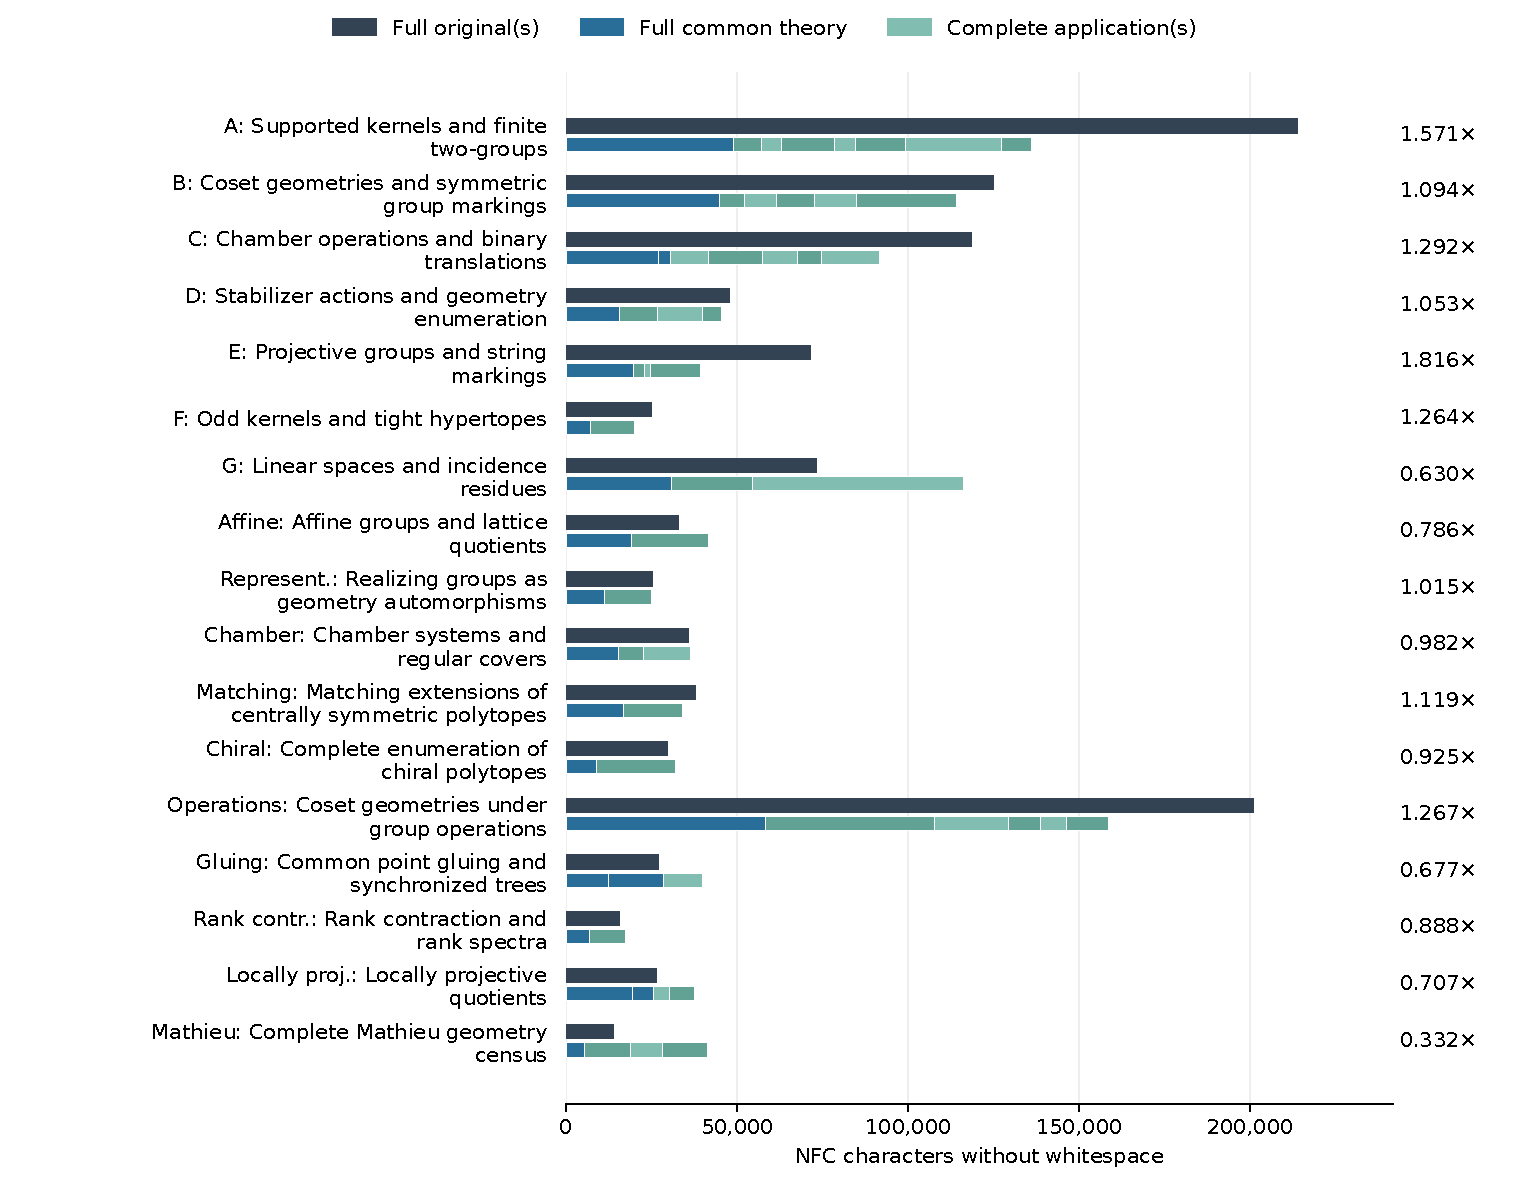
\includegraphics[width=\linewidth]{whole_topics.pdf}\end{center}
All earlier common and application boundaries remain unchanged. Locally projective pays 7+5 common pages and both applications (2+3 pages). Mathieu pays its two-page common paper and all 5+10+9 application pages. Companion tables are complete papers in these denominators, not free outputs. Text length is not minimum proof complexity or originality.
\newpage
\textbf{Complete programs and prior acquisition.}
The written comparison remains first. These alternatives add the entire declared code representation and any separately measured mandatory data. Raw and printed code are never added together. The new data column is separate from code in both denominators.
\begin{center}\tabsetup\begin{tabular}{lrrrrrr}\toprule
Topic & Printed code & Data & With printed & Raw code & With raw & Upfront\\\midrule
A & 54,210 & -- & 1.124 & 52,807 & 1.132 & 103,269 \\
B & 13,170 & -- & 0.981 & 12,330 & 0.987 & 58,075 \\
C & 20,933 & -- & 1.052 & 19,937 & 1.061 & 51,370 \\
D & 27,070 & -- & 0.660 & 26,185 & 0.668 & 42,702 \\
E & 7,565 & -- & 1.523 & -- & -- & 27,355 \\
F & 8,837 & -- & 0.875 & 8,061 & 0.899 & 15,955 \\
G & 53,018 & -- & 0.433 & 50,184 & 0.440 & 83,946 \\
Affine & 17,250 & -- & 0.556 & 16,682 & 0.561 & 36,320 \\
Represent. & 9,025 & -- & 0.746 & 8,310 & 0.762 & 20,313 \\
Chamber & 7,677 & -- & 0.811 & 6,401 & 0.835 & 22,876 \\
Matching & 4,998 & -- & 0.976 & 4,408 & 0.991 & 21,730 \\
Chiral & 11,940 & -- & 0.674 & 11,090 & 0.687 & 20,771 \\
Operations & -- & -- & -- & 403,848 & 0.357 & 462,063 \\
Gluing & 13,371 & -- & 0.508 & 12,768 & 0.513 & 41,787 \\
Rank contr. & 2,925 & -- & 0.761 & 2,501 & 0.777 & 9,862 \\
Locally proj. & 22,695 & 28,574 & 0.299 & 22,104 & 0.301 & 76,767 \\
Mathieu & 31,244 & 48,686 & 0.113 & 30,489 & 0.114 & 85,446 \\
\bottomrule\end{tabular}\end{center}
Upfront means the whole common theory, complete printed code when available, and separately measured mandatory data. A dash in the Data column for an older record does not mean its external data is free; those historical boundaries remain unchanged. Locally projective adds all 28,574 data characters (39,150 literal bytes), and Mathieu all 48,686 (83,965 bytes), to both code alternatives. For Operations it uses all twenty-three whole mathematical/validation files plus both required decoding drivers. Its complete printed route is unavailable: the two partial appendices cover only four named raw files. Operations conditionals also assume acquisition of all required external data, separately inventoried as 21,960,689 representation bytes and 2,516,249 listed installed bytes. Byte storage is not added to character units. Large witnesses are not discounted.

E retains its separate optional-validation sensitivity: another 5,173 characters gives a program-inclusive factor of 1.372. No unadmitted raw-code alternative is invented for E.

\textbf{Roles.} A includes five full files. B includes a finite premise, two validations and an auxiliary example. C includes its three complete GAP files, counting the identical shared construction once within C and retaining its exhaustive census. D includes five required and three diagnostic programs. E separates its required program from optional validation. F's three programs and Representation's two are validations. G retains four finite computations, two certificate bridges and seven validations. Affine retains six mathematical programs; Chamber one required and one diagnostic program; Matching its census; Chiral enumeration all three files. Operations includes seventeen finite proof/witness files, six validations and both required decoders. Gluing pays all three complete validation programs, with three drivers and two partial Lean files separate. Rank contraction keeps its whole finite-example program, driver and four partial Lean declarations separate. Locally projective requires six complete programs and whole historical reconciliation JSON; Mathieu requires seven programs and both entire JSON inputs. Their three drivers each and eleven/ten generated outputs are separate; neither has Lean declarations. Other inventories stay unchanged.

\textbf{Limits.} Complete external proofs, unprovided historical software, full graphics and end-to-end formalization have unknown costs, not zero. Every topic retains its underlying multi-unit and source-cover sensitivities. B's source costs are unchanged from the prior edition. This table does not compare a theorem closure with a complete original or use a node-count ratio.
\newpage
\textbf{Every complete application after full acquisition.}
The entire common theory and all declared software/data have already been acquired. Every local page is charged, including context, references and companions. DG2 includes all N006 papers; MC1 includes all 24 Mathieu application pages.
\begin{center}\tabsetup\renewcommand{\arraystretch}{1.03}\begin{tabular}{lllrrr}\toprule
Topic & Original & Application & Source cost & Application cost & Conditional\\\midrule
A & L032 & A1 & 16,558 & 8,212 & 2.016 \\
A & L034 & A2 & 21,433 & 5,784 & 3.706 \\
A & F016 & A3 & 43,983 & 15,419 & 2.853 \\
A & F013 & A4 & 25,562 & 6,224 & 4.107 \\
A & L035 & A5 & 51,019 & 14,498 & 3.519 \\
A & N009 & A6 & 36,824 & 28,114 & 1.310 \\
A & L128 & A7 & 18,424 & 8,768 & 2.101 \\
B & N001 & B1 & 14,519 & 7,371 & 1.970 \\
B & N003 & B2 & 17,780 & 9,155 & 1.942 \\
B & N008 & B3 & 18,009 & 11,132 & 1.618 \\
B & L030 & B4 & 22,704 & 12,286 & 1.848 \\
B & L040 & B5 & 51,894 & 29,321 & 1.770 \\
C & L088 & C1 & 13,166 & 11,311 & 1.164 \\
C & N013 & C2 & 27,361 & 15,815 & 1.730 \\
C & L108 & C3 & 12,849 & 10,075 & 1.275 \\
C & F014 & C4 & 20,577 & 6,962 & 2.956 \\
C & L068 & C5 & 44,480 & 17,085 & 2.603 \\
D & L066 & D1 & 20,916 & 10,989 & 1.903 \\
D & L074 & D2 & 20,661 & 13,367 & 1.546 \\
D & L104 & D3 & 6,317 & 5,499 & 1.149 \\
E & L083 & E1 & 20,885 & 3,002 & 6.957 \\
E & L079 & E2 & 20,908 & 1,855 & 11.271 \\
E & L021 & E3 & 29,582 & 14,656 & 2.018 \\
F & L014 & F1 & 25,115 & 12,744 & 1.971 \\
G & L009 & G1 & 49,891 & 23,544 & 2.119 \\
G & L092 & G2 & 23,308 & 61,663 & 0.378 \\
Affine & L012 & AF1 & 32,767 & 22,638 & 1.447 \\
Represent. & F010 & R1 & 25,348 & 13,688 & 1.852 \\
Chamber & L008 & H1 & 21,784 & 7,571 & 2.877 \\
Chamber & N016 & H2 & 14,018 & 13,683 & 1.024 \\
Matching & F015 & M1 & 37,951 & 17,168 & 2.211 \\
Chiral & L028 & CE1 & 29,599 & 23,171 & 1.277 \\
Operations & N005 & OP1 & 122,002 & 49,595 & 2.460 \\
Operations & N006 & DG2 & 56,001 & 38,479 & 1.455 \\
Operations & N007 & DG1 & 22,888 & 12,305 & 1.860 \\
Gluing & L010 & GL1 & 27,081 & 11,565 & 2.342 \\
Rank contr. & L037 & RC1 & 15,530 & 10,555 & 1.471 \\
Locally proj. & L084 & LP1 & 2,071 & 4,857 & 0.426 \\
Locally proj. & L095 & LP2 & 24,419 & 7,109 & 3.435 \\
Mathieu & L073 & MC1 & 13,736 & 35,862 & 0.383 \\
\bottomrule\end{tabular}\end{center}
All fifteen previous topic records remain unchanged. Three complete applications are added. Forty measured originals is not inferred to be the total recovered; no scientific credit is assigned.
\newpage
\textbf{Individual source and application costs: first seventeen originals.}
Dark bars show complete original texts; green bars show complete applications. Factors at right assume full prior acquisition. The source and replacement bars share the same scale within each chart.
\begin{center}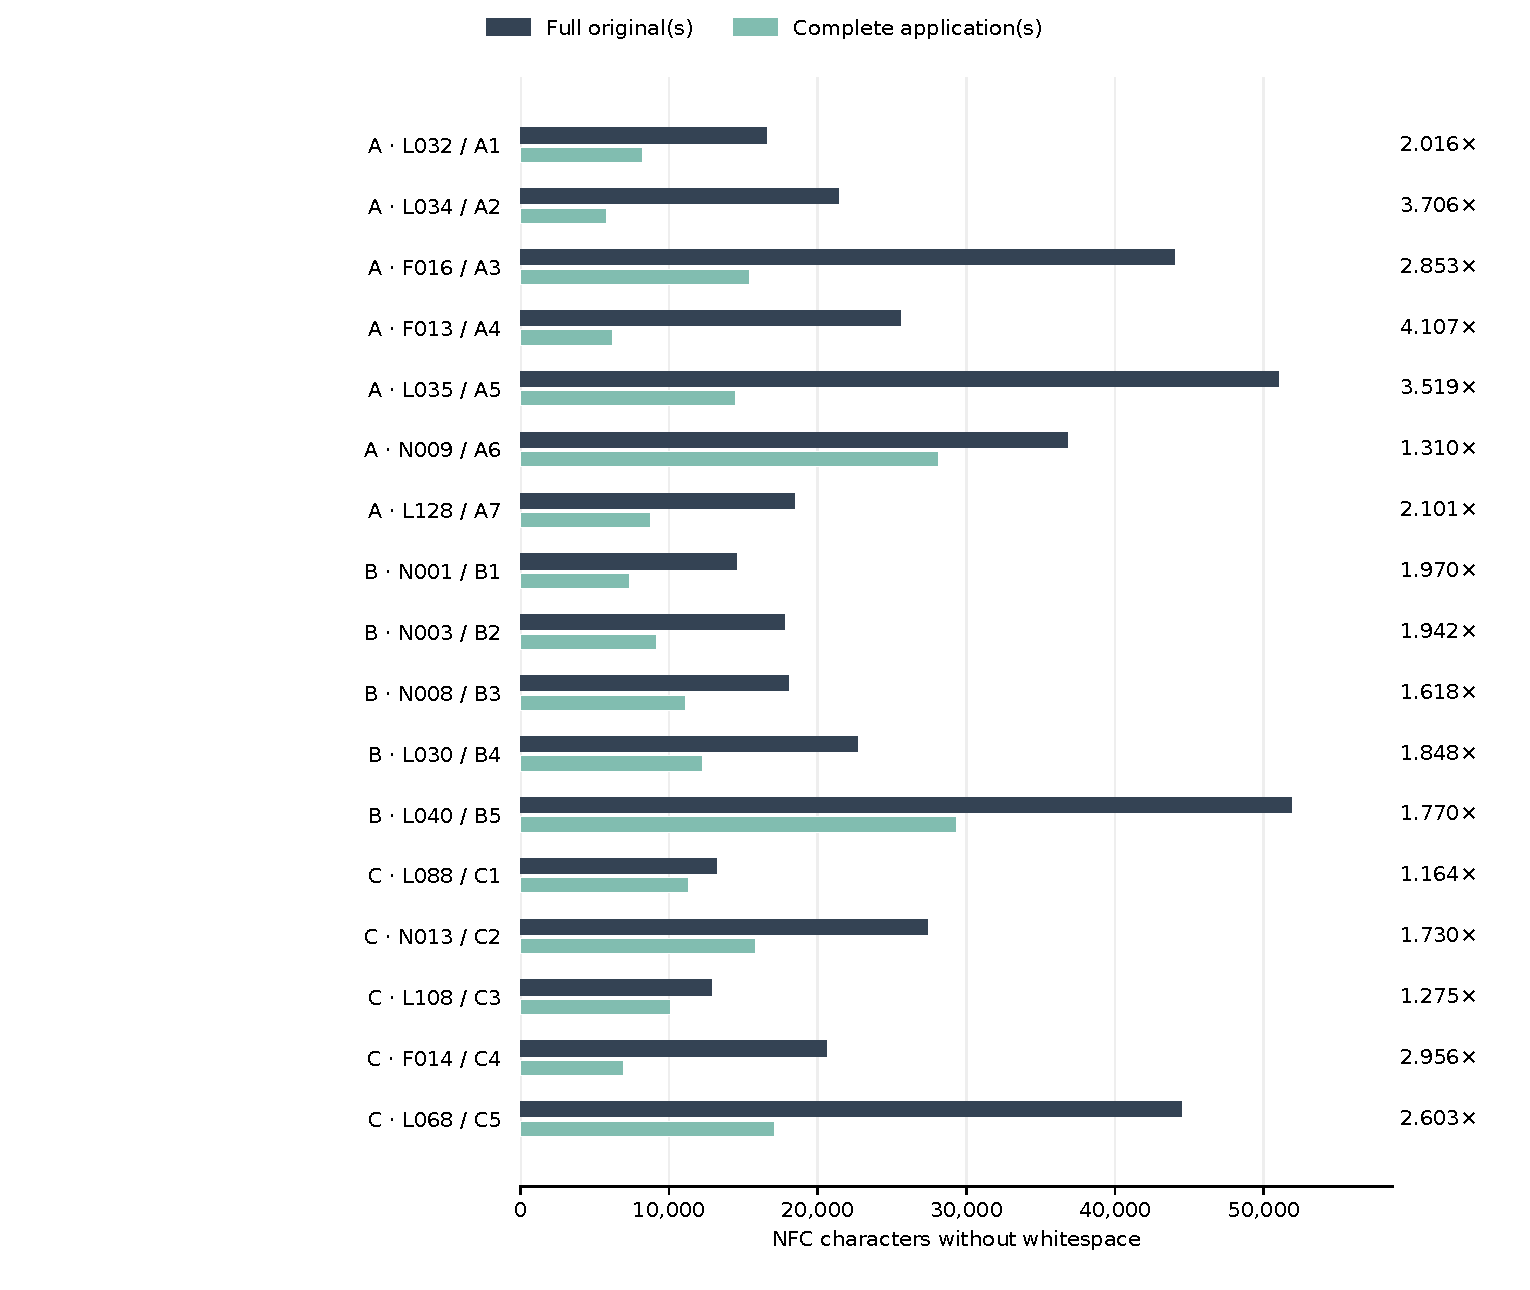
\includegraphics[width=\linewidth]{conditional_1.pdf}\end{center}
Source IDs remain stable catalogue cross-references. LP1 is the complete 2006 erratum; LP2 uses the full fifteen-page 2003 arXiv edition, not the unseen journal text. Their source-column corrections remain qualified. MC1 gives the corrected 81/431-class census and all 431 literal-row dispositions, not unavailable historical \texttt{geo[]} identities. Its 48-page predecessor is retained notation, not a newly recovered original.
\newpage
\textbf{Individual source and application costs: remaining twenty-three originals.}
The same conventions apply. LP1 and LP2 assume acquisition of the whole Locally projective proof, common tables, all six programs and mandatory JSON. The final MC1 bar contains all three Mathieu application papers, after whole common theory, all seven programs and both JSON inputs. Other topics remain separately paid; no overlap is deducted.
\begin{center}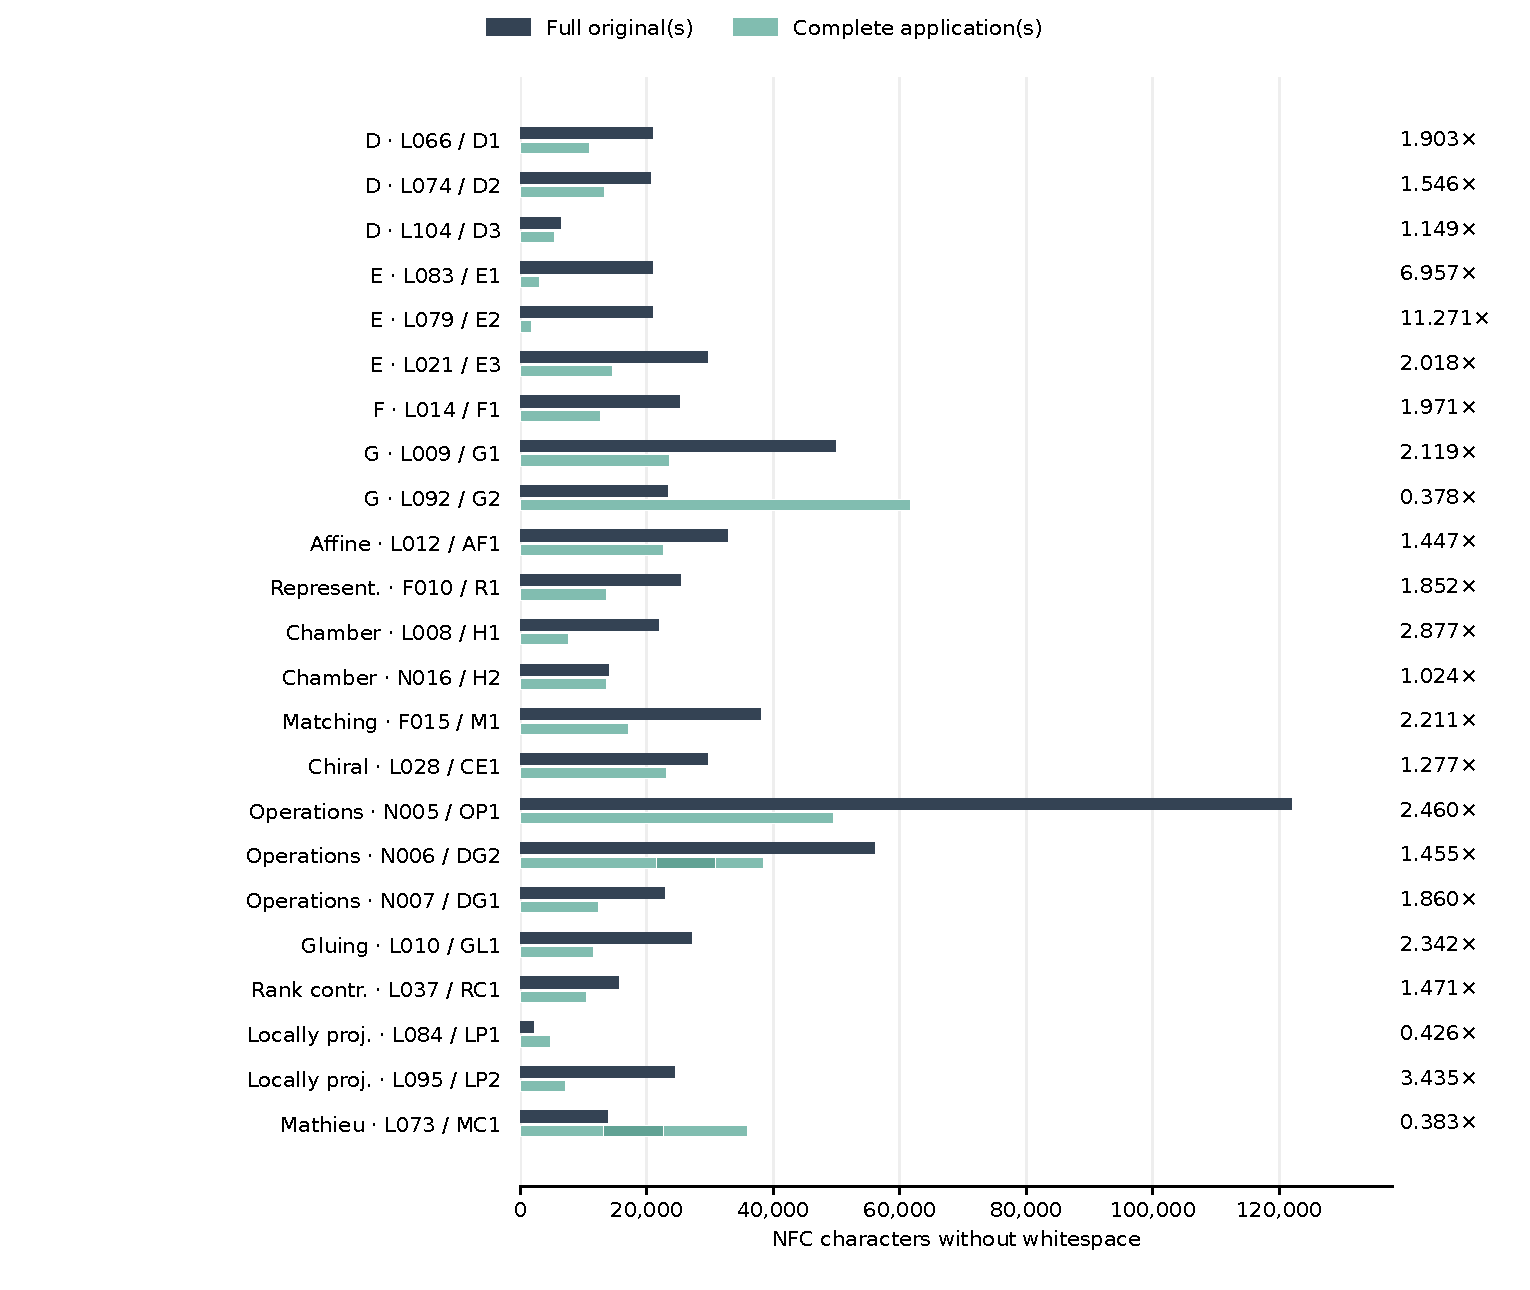
\includegraphics[width=\linewidth]{conditional_2.pdf}\end{center}
\textbf{Data and provenance.} Exact integers and rational comparisons are in \texttt{results.json}, \texttt{topics.csv} and \texttt{applications.csv}. The protocol pins committed unchanged numerical/admission records and the two new frozen numerical packets and their distinct root acceptances directly. No primary text is copied or extracted. Bar segments use complete document costs, not theorem counts. Distinct review is required before this overview becomes the public current edition.
\end{document}
